\documentclass[11pt]{article}

% ============================================================================
% Paper 3 -- Retention under Query-Axis Top-K Sparse Attention
% arXiv / Zenodo preprint source.  Compile: pdflatex x2.
% ============================================================================

\usepackage[utf8]{inputenc}
\usepackage[T1]{fontenc}
\usepackage{amsmath,amssymb,amsthm}
\usepackage{graphicx}
\usepackage{booktabs}
\usepackage{geometry}
\usepackage{xcolor}
\usepackage[hidelinks]{hyperref}
\usepackage{caption}
\usepackage{enumitem}
\usepackage{authblk}

\geometry{a4paper, margin=1in}
\captionsetup{font=small, labelfont=bf}
\setlist{nosep, leftmargin=1.4em}

\newcommand{\keff}{k_{\mathrm{eff}}}
\newcommand{\Kcrit}{K_{\mathrm{crit}}}
\newcommand{\uQ}{\mathbf{u}_Q}

\title{\bfseries No Critical Key Budget in Query-Axis Top-$K$ Sparse Attention:\\
Long-Context Retention Is Bounded by the Base Model, Not the Compressor}

\author[1]{Evgenii Vyaltsev\thanks{ORCID 0009-0004-3712-6798. Correspondence: handle \texttt{@seqe\_phi}.}}
\author[1]{Daniil Vyaltsev}
\affil[1]{Independent Researcher}

\date{June 2026}

\begin{document}
\maketitle

\begin{abstract}
\noindent
Top-$K$ sparse attention is widely deployed to extend context and reduce memory,
on the implicit premise that there exists a key budget below which long-context
ability collapses. We test that premise directly. Using a training-free,
exact-ranking query-axis selector (top-$K$ by $\langle\uQ,K_i\rangle$,
$\uQ=Q/\lVert Q\rVert$) on Llama-3.2-1B, we run a staircase of pre-registered
retrieval-under-competition gates with paired confidence intervals, a three-way
failure attribution (\textsc{correct} / \textsc{wrong-needle} / \textsc{starvation}),
and a needle-in-top-$k$ selection probe. The decisive experiment \emph{decouples}
the absolute key budget $\keff$ from context length $N$ by driving $\keff$ to fixed
absolute targets while sweeping $N$. We find that \textbf{$\keff$ is nearly inert}:
a $4\times$ swing of the budget over $[1300,5200]$ moves retrieval accuracy by
$\le 0.03$ at any $N$, refuting the existence of an absolute ``critical semantic
capacity'' $\Kcrit$. The long-context limit is instead the base model's own
length-driven \emph{disambiguation} failure --- the same needle is selected into
the top-$k$ ever more often as the budget grows, yet the answer does not improve,
and full (dense) attention degrades identically. A cross-model gate
(Qwen2.5-3B, Llama-3.2-3B; kernel port validated bitwise-exact against a
pure-PyTorch reference) shows the picture is general across two architecture
families and a $3\times$ capacity span: $\Kcrit$ does not emerge with capacity;
instead, capacity \emph{raises the ceiling} (the ``selected-yet-wrong'' fraction at
$N{=}32\mathrm{K}$ falls $0.37\!\to\!0.23\!\to\!0.18$). Finally, a pre-registered
causal probe that up-weights the needle's attention within a fixed selected set
recovers most failures, but \emph{plain re-delivery of the same fact recovers more}
($100\%\ge 80\%$): the correctness bottleneck is downstream of attention --- a
delivery/salience deficit plus the weights --- not a computation attention performs.
We conclude that within the practical operating regime there is \emph{no efficiency
cliff in the compressor}; top-$K$ retains as well as dense right up to the point
where the task defeats dense itself. Implications: for off-the-shelf models the
actionable lever for ``smarter'' is capacity (or better delivery), not the key
budget; the safe operating coverage is $c\gtrsim 0.10$ to $128\mathrm{K}$.
All claims are scoped to retrieval-selection (greedy, no chain-of-thought);
multi-hop synthesis floors on these bases and is deferred.
Code, raw per-prompt logs, and pre-registrations are released.
\end{abstract}

\section{Introduction}
\label{sec:intro}

A perplexity-preserving compressor is not the same thing as a
retention-preserving one. A sparse-attention engine can match dense perplexity
while silently dropping the one distant key on which a particular answer hinges:
iso-PPL $\neq$ iso-retrieval $\neq$ iso-reasoning. This paper isolates the middle
term --- \emph{does top-$K$ sparse decode preserve dependence on a distant
\textbf{required} key under competition?} --- and, in doing so, refutes a specific
folk hypothesis about \emph{why} long-context ability eventually breaks.

The hypothesis we test, which we call the \emph{Critical Semantic Capacity}
conjecture, is the natural reading of selection-based sparse attention: there is an
absolute key budget $\Kcrit$ such that for $\keff>\Kcrit$ retention holds
\emph{independent of $N$}, and below it the top-$k$ selector starts grabbing the
wrong key (mis-selection). If true, $\Kcrit$ would be the single number a
practitioner needs, and pushing $N$ would be safe as long as $\keff$ stays above it.

We show this conjecture is false for the systems we study, and we show \emph{what
replaces it}. Our contributions:
\begin{enumerate}
\item \textbf{A decoupling experiment (\S\ref{sec:keff}).} Holding $\keff$ at fixed
\emph{absolute} targets $\{1300,2000,2600,3500,5200\}$ while sweeping
$N\in\{32\mathrm{K},65\mathrm{K},98\mathrm{K},131\mathrm{K}\}$ separates an
absolute-budget law from a coverage law from a length effect. The budget axis is
\emph{inert} (accuracy range $\le 0.03$ across a $4\times$ swing at every $N$);
the same budget $\keff{=}5200$ holds at $32\mathrm{K}$ yet fails at $65\mathrm{K}$.
$\Kcrit$ does not exist.
\item \textbf{A selection/answer dissociation.} A reconstructed needle-in-top-$k$
probe rises monotonically with the budget --- the needle \emph{is} selected more
often --- while accuracy does not move. Even when the needle is in the top-$k$ the
model picks a wrong same-class competitor. The bottleneck is disambiguation, not
selection.
\item \textbf{Cross-model generality (\S\ref{sec:cross}).} On Qwen2.5-3B and
Llama-3.2-3B (two families, $3\times$ capacity), with a kernel port validated
bitwise-exact against the reference, $\Kcrit$ still does not emerge. Retention
transfers; capacity instead lowers the selected-yet-wrong fraction and raises dense
accuracy. We name this \emph{capacity-shifts-ceiling}.
\item \textbf{A causal probe of attention's role (\S\ref{sec:causal}).} Up-weighting
the needle's attention logits within a fixed selected set is a real,
needle-specific, directional lever on correctness --- yet plain re-delivery of the
fact recovers at least as much. Per pre-registration this is \emph{transport, not
computation}: the failure is downstream of attention.
\end{enumerate}

The honest headline is stronger than the conjecture it replaces because it is a
falsifiable null that survived: \emph{there is no compressor cliff over the
practical regime}. Top-$K$ with $\keff\gtrsim 1300$ retains as well as dense up to
the point where the base model's length-driven disambiguation limit defeats dense
itself.

\section{Related work}
\label{sec:related}

\paragraph{Selection-based sparse attention.}
Training-free KV selection spans token-level
(StreamingLLM~\cite{xiao2023streaming}, H2O~\cite{zhang2023h2o},
SnapKV~\cite{li2024snapkv}), block/page-level
(InfLLM~\cite{xiao2024infllm}, Quest~\cite{tang2024quest}), ANN-based
(RetrievalAttention~\cite{liu2024retrieval}), and low-rank
(Loki~\cite{singhania2024loki}). Trained selectors --- DeepSeek
DSA~\cite{deepseek2025v32}, NSA~\cite{yuan2025nsa}, MoBA --- give stronger numbers
but require continued pre-training. Our selector is training-free and \emph{exact}
in ranking (\S\ref{sec:method}); the present paper is not about the selector's
quality (established elsewhere) but about \emph{what limits retention} when such a
selector is used.

\paragraph{Top-$k$ theory and attention concentration.}
A recent line gives error bounds and entropy readings for top-$k$ truncation:
a total-variation factorization of the truncation
error~\cite{tvtopk2025}, the observation that low-entropy states are better suited
to top-$k$ decoding~\cite{nativetopk2025}, and a critical-scaling account in which
attention logits scale as $\beta_n\asymp\log n$ and mass concentrates on a
sublinear-but-nontrivial set~\cite{criticalscaling2025}. Concurrent work reports
that attention concentration in trained models is a \emph{learned}, not
architectural, property~\cite{condensate2026}. These predict that \emph{some}
distant mass is always retained and that the effective support grows sublinearly;
our results are consistent with that and add the orthogonal, empirical finding that
once the budget exceeds the recency floor, \emph{the budget itself stops mattering}
and the limit is the model's disambiguation.

\paragraph{Long-context evaluation.}
Needle-in-a-haystack and ``lost-in-the-middle'' studies~\cite{liu2024lost} establish
that retrieval accuracy depends on position and length even for dense attention.
Our dense arm reproduces a length-driven degradation; the contribution here is
attributing it to the base model rather than to the sparsifier, via a matched
dense control and a three-way failure decomposition.

\paragraph{Matched-magnitude controls.}
The causal probe in \S\ref{sec:causal} follows a matched-magnitude intervention
discipline~\cite{matchedcontrols2026}: a candidate cause is compared against a
control of equal perturbation magnitude, and a pre-registered null closes the
direction. This is the methodology that, in our own prior program, falsified a
spectral-mechanism hypothesis; we apply it here to attention weight as a cause of
correctness.

\section{Method and experimental design}
\label{sec:method}

\paragraph{Selector.}
For query $Q$ and key $K_i$, ranking by the unit-normalized projection is
order-identical to ranking by the raw score,
\begin{equation}
\langle Q,K_i\rangle > \langle Q,K_j\rangle
\;\Longleftrightarrow\;
\langle \uQ,K_i\rangle > \langle \uQ,K_j\rangle,
\qquad \uQ=\frac{Q}{\lVert Q\rVert_2},
\label{eq:thm1}
\end{equation}
so selecting the top-$\keff$ keys by $\langle\uQ,K_i\rangle$ is exact (no learned
parameters, no lossy approximation). The budget follows a coverage floor $c$,
\begin{equation}
\keff = \min\!\big(N,\ \max(64,\ \lfloor c\,N\rfloor)\big)\quad\text{(even-rounded)},
\label{eq:keff}
\end{equation}
with recency window $k_{\mathrm{window}}=64$. All selection is fp32-softmax;
the Triton kernel is validated equal to a pure-PyTorch reference.

\paragraph{Two arms (matched control).}
\textsc{dense}: full SDPA decode (\texttt{enable\_dcr=False}), $c$-independent,
decoded once per prompt. \textsc{sparse}: query-axis top-$K$ at the $c$ realizing
the target $\keff$. Route counters are checked per cell (sparse all-DCR
$\text{sdpa}=0$; dense all-SDPA $\text{dcr}=0$); a silent SDPA fallback invalidates
a cell. The prefill-confound is re-confirmed each run: the shared dense prefill's
first generated token carries zero code digits, so every digit of an answer is
emitted by the arm's own decode.

\paragraph{Task and scoring.}
Retrieval-under-competition: $K{=}16$ planted ``codes'', a query that selects one by
a \emph{semantic} attribute (no verbatim id, removing the lexical-lookup escape
hatch), and $K{-}1$ same-class distractors at high density. The first complete
7-digit code is the committed answer, scored three ways:
\textsc{correct}; \textsc{wrong-needle} (a \emph{different planted} code ---
mis-selection); \textsc{starvation} (hallucinated other-code or miss --- too few
keys / degeneration). \textsc{wrong-needle} is never collapsed into miss. We report
the differential vs.\ dense for each mode separately, each with a paired bootstrap
CI ($10^4$ resamples).

\paragraph{Selection probe (needle-in-top-$k$).}
Per prompt, at the answer-emitting step, we record whether the needle span's
query-axis score rank is within $\keff$ (mean over layers/heads, thresholded). This
separates ``the needle was selected'' from ``the answer was right''. A cell that
passes while the probe has dropped is robust-but-via-leak, not a clean selection
pass, and is flagged.

\paragraph{Pre-registration.}
Every gate fixes its grid, thresholds, monotone-neighbour rule, and verdict map
\emph{before} execution; none is tunable after. A cell is \emph{informative} only if
$\mathrm{acc}_{\textsc{dense}}\in[0.30,0.95]$ (ceilinged/floored cells are excluded
and reported). \textsc{fail} if $\mathrm{CI}_{\text{upper}}(\text{dense}-\text{sparse})>0.05$
or $\mathrm{CI}_{\text{upper}}(\text{wrong}_s-\text{wrong}_d)>0.05$. Seed $=20260531$
throughout; greedy decode; bf16 weights with fp32 softmax. Hardware: a single
RTX~4060~Ti (16\,GB).

\section{Warm-up gates: where the task does and does not bite}
\label{sec:warmup}

A single salient needle is never dropped: at $N\in\{8\mathrm{K},32\mathrm{K},
128\mathrm{K}\}$ and four depths, dense $=$ sparse $=1.000$ (a ceiling --- necessary,
not sufficient). A multi-needle task with \emph{unique} ids is also uninformative:
distinct ids make the query a lexical lookup, distractors do not compete, and sparse
is byte-identical to dense (all cells ceiling). A controlled illustration of the
statistical discipline: one pilot cell read $0.80$ at $n{=}5$ and regressed to
$0.99$ at $n{=}100$ --- the paired-CI + monotone-neighbour rule correctly rejected
the phantom boundary that a point threshold at small $n$ would have reported.

The task bites only under \emph{soft} disambiguation (semantic attribute, or
near-duplicate ids sharing $3/4$ digits). There, with real dense headroom
(dense $0.40$--$0.93$), every informative cell holds at $c{=}0.15$ (zero
\textsc{fail}s), and crucially \emph{sparse co-tracks dense's own errors}: in hard
cells dense itself has a high wrong-needle rate and sparse reproduces the rate and
pattern rather than adding selection failures of its own. Sweeping $c$ down to
$0.02$ moves the only boundary into $N$, not $c$: cells at $N\le 32\mathrm{K}$ hold
to $c{=}0.02$, while $N{=}131\mathrm{K}$ degrades --- and at that extreme a majority
of \emph{correct} answers occur with the needle \emph{not} in the top-$k$
(leak/redundancy), so accuracy ceases to indicate the memory mechanism at very low
coverage. This motivates the decoupling experiment: from a single failing corner
($c{=}0.02$, $N{=}128\mathrm{K}$, where $\keff{\approx}2600$) one cannot tell an
absolute-budget law from a coverage law from a length effect, because $c$ and $N$
moved together.

\section{The key budget is inert; there is no $\Kcrit$}
\label{sec:keff}

We drive $\keff$ \emph{directly} to fixed absolute targets
$\{1300,2000,2600,3500,5200\}$ (choosing $c=\keff/N$ per cell, verifying
Eq.~\ref{eq:keff} reproduces the target to $\pm 2$, $\text{window\_floored}=0$), and
read \textsc{fail} across $N$ at each fixed budget and across budgets at each fixed
$N$. Within-run pairing is airtight (prompt identity asserted across all $\keff$ in
a cell; realized $\keff$ equals target exactly).

Table~\ref{tab:keff} and Fig.~\ref{fig:keff}/\ref{fig:dissoc} give the result.
\begin{table}[t]
\centering
\small
\caption{Semantic $K{=}16$, Llama-3.2-1B. $\mathrm{acc}_{\textsc{sparse}}$ at each
absolute $\keff$, with dense in brackets; \emph{accRange} is the max$-$min across the
$4\times$ budget swing; \emph{nit} is the needle-in-top-$k$ rate
(min$\to$max over $\keff$). Numbers recomputed from per-prompt logs.}
\label{tab:keff}
\begin{tabular}{lcccccccl}
\toprule
$N$ & dense & 1300 & 2000 & 2600 & 3500 & 5200 & accRange & nit ($\to$) \\
\midrule
32K  (inf.) & 0.62 & 0.61 & 0.60 & 0.62 & 0.62 & 0.62 & 0.02 & $0.66\!\to\!0.86$ \\
65K  (inf.) & 0.49 & 0.41 & 0.43 & 0.43 & 0.44 & 0.45 & 0.04 & $0.57\!\to\!0.75$ \\
98K  (floor)& 0.28 & 0.30 & 0.28 & 0.29 & 0.26 & 0.26 & 0.04 & $0.46\!\to\!0.62$ \\
131K (inf.) & 0.40 & 0.40 & 0.42 & 0.42 & 0.42 & 0.42 & 0.02 & $0.45\!\to\!0.61$ \\
\bottomrule
\end{tabular}
\end{table}

\begin{figure}[t]
\centering
\begin{minipage}{0.49\textwidth}\centering
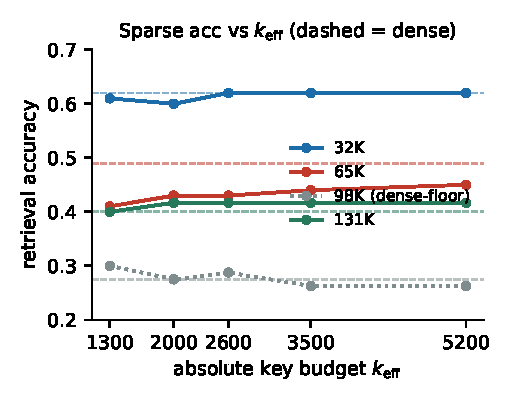
\includegraphics[width=\linewidth]{figures/fig1_keff_inert.pdf}
\caption{The budget axis is flat. A $4\times$ swing of $\keff$ barely moves
accuracy at any $N$. The \emph{same} budget $\keff{=}5200$ holds at 32K
(diff $0.00$) yet fails at 65K (diff $+0.04$, $\mathrm{CI}[+0.01,+0.08]$) --- a
fixed-$\Kcrit$ law would require it to hold at every $N$.}
\label{fig:keff}
\end{minipage}\hfill
\begin{minipage}{0.49\textwidth}\centering
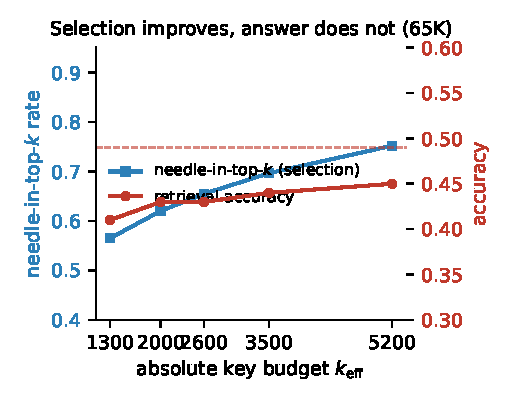
\includegraphics[width=\linewidth]{figures/fig2_dissociation.pdf}
\caption{Selection improves, the answer does not (65K). The needle is captured in
the top-$k$ ever more often as the budget grows (left axis), yet accuracy is flat
(right axis): the captured needle does not help because the model cannot
disambiguate among the $K{=}16$ competitors.}
\label{fig:dissoc}
\end{minipage}
\end{figure}

\paragraph{$\Kcrit$ is falsified.}
A fixed absolute $\Kcrit$ requires a budget far above $2600$ to hold at \emph{every}
$N$. It does not: $\keff{=}5200$ holds at $32\mathrm{K}$ (diff $0.00$) but fails at
$65\mathrm{K}$ (diff $+0.04$, $\mathrm{CI}[+0.01,+0.08]$, McNemar $b\!\gg\!c$). Nor is
it a coverage law: $c{=}0.04$ ($\keff{=}1300$ @ $32\mathrm{K}$) holds while
$c{=}0.079$ ($\keff{=}5200$ @ $65\mathrm{K}$) fails --- a \emph{lower} coverage holding
while a \emph{higher} one fails rules out a fixed-coverage onset. The auto-classifier
labelled the surface ``mixed''; on review this is the mechanical artifact of two
noise-driven points (65K fails by a flat $\sim\!0.05$ gap at all budgets; the 131K
$\keff{=}1300$ ``fail'' is an $n{=}60$ CI artifact with point-diff $0.00$). The
substantive reading is decisive: \textbf{the budget is inert and there is no
$\Kcrit$.}

\paragraph{The limit is the base model.}
Dense's own wrong-needle rate \emph{rises with $N$}
($0.37\!\to\!0.41\!\to\!0.52$, peaking $0.58$ at $98\mathrm{K}$): full attention
itself increasingly grabs the wrong same-class competitor as filler grows. Even when
the needle is in the top-$k$, the model picks wrong (e.g.\ 65K @ $\keff{=}5200$:
in-and-correct $43$ vs.\ in-and-wrong $55$). The sparse penalty (dense$-$sparse) is
$\le 0.08$, budget-insensitive, and visible only at $65\mathrm{K}$ where dense still
has headroom above its wrong-needle floor; at $131\mathrm{K}$ dense has already
collapsed toward that floor, so sparse cannot fall further and ``holds'' trivially.
The shape is smooth, not a phase transition --- no abrupt fail between adjacent
budgets at any $N$. A near-duplicate branch (doubled $n$) finds no aliasing: the
wrong-needle differential CI contains $0$ at $32\mathrm{K}$ and is negative at
$131\mathrm{K}$ (sparse has \emph{less} wrong-needle than dense). Mis-selection is
not the established failure mode; the base model's disambiguation is.

\section{Cross-model: the picture is general, and capacity raises the ceiling}
\label{sec:cross}

\paragraph{Port validity (hard precondition).}
We removed a 1B-specific GQA hardcode from the selection kernel (generalizing the
query-head unroll to any GQA ratio; dropping head-dim asserts; replacing a stable
argsort with a top-$k$ + fp64 index-monotone tie-break that reproduces the
reference's smaller-index-wins rule). The result is validated \emph{bitwise-exact}
against the pure-PyTorch reference ($\max|\Delta O|=0.0$, index agreement $1.0$) at
GQA ratios $4$/$8$/$3$ (Llama-1B / Qwen-3B / Llama-3B), and the full dense forward is
bit-identical to vanilla HF ($\max|\Delta\text{logit}|=0.0$) for both 3B models.
Results are therefore not port-confounded. A separate iso-PPL check on general text
at $c{=}0.15$ shows Llama-3.2-3B is more sparse-sensitive on \emph{perplexity}
($+2.74\%$, CI excludes $0$) than Qwen2.5-3B ($+0.27\%$, CI contains $0$); this is a
genuine model property, and notably it does \emph{not} translate to retrieval
failure (below).

\paragraph{Gate B (same absolute budgets, $n{=}100$, $K{=}16$).}
\begin{table}[t]
\centering
\small
\caption{Cross-model semantic retrieval, $n{=}100$. $\mathrm{acc}_{\textsc{sparse}}$
at each $\keff$, dense in brackets; \emph{in\&wrong} is the needle-selected-yet-wrong
fraction. Recomputed from per-prompt logs. ($N$ memory-bounded: Qwen $\le 65\mathrm{K}$,
Llama-3B $\le 49\mathrm{K}$ on 16\,GB.)}
\label{tab:cross}
\begin{tabular}{llccccccc}
\toprule
model & $N$ & dense & 1300 & 2000 & 2600 & 3500 & 5200 & accRange / in\&wrong\\
\midrule
Qwen2.5-3B   & 32K & 0.75 & 0.79 & 0.78 & 0.76 & 0.78 & 0.76 & 0.03 / 0.23\\
Qwen2.5-3B   & 65K & 0.35 & 0.33 & 0.33 & 0.34 & 0.33 & 0.34 & 0.01 / 0.55\\
Llama-3.2-3B & 32K & 0.81 & 0.82 & 0.82 & 0.82 & 0.81 & 0.81 & 0.01 / 0.18\\
Llama-3.2-3B & 49K & 0.82 & 0.80 & 0.81 & 0.83 & 0.83 & 0.82 & 0.03 / 0.18\\
\bottomrule
\end{tabular}
\end{table}

\begin{figure}[t]
\centering
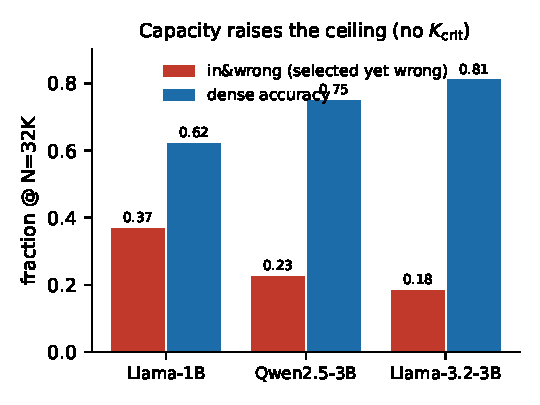
\includegraphics[width=0.52\textwidth]{figures/fig3_capacity.pdf}
\caption{Capacity-shifts-ceiling at $N{=}32\mathrm{K}$. Larger models do not reveal a
$\Kcrit$ (the budget stays inert, Table~\ref{tab:cross}); they disambiguate better ---
the selected-yet-wrong fraction falls $0.37\!\to\!0.23\!\to\!0.18$ and dense accuracy
rises $0.62\!\to\!0.75\!\to\!0.81$.}
\label{fig:cap}
\end{figure}

The budget is inert on both 3B models (accRange $0.01$--$0.03$); retention transfers
(every informative cell $\mathrm{CI}_{\text{upper}}\le 0.05$); the failure mode is
not budget-driven. What capacity changes is the \emph{ceiling}: at matched
$N{=}32\mathrm{K}$ the selected-yet-wrong fraction falls
$0.37$ (1B) $\to 0.23$ (Qwen-3B) $\to 0.18$ (Llama-3B), with dense accuracy rising in
lockstep (Fig.~\ref{fig:cap}). $\Kcrit$ does not emerge with capacity or across
families; the long-context bottleneck is disambiguation-in-weights, and more
capacity improves that bottleneck rather than replacing it with a key-budget law. We
summarize the three verdicts as \textbf{no-$\Kcrit$ / weights-bound (universal) /
capacity-shifts-ceiling}. This is a transfer result over three models and two
families, not yet a scaling law in (model, depth, $N$, $\keff$); more models are the
natural next gate.

\section{Is attention computing the answer, or only delivering it?}
\label{sec:causal}

The dissociation in \S\ref{sec:keff} (needle selected yet answer wrong) raises a
causal question the selection probe cannot settle: is the needle's attention
\emph{weight} a cause of correctness, or merely an indicator of what the weights
already decided? We manipulate the one lever no prior gate touched --- the needle's
attention weight \emph{within a fixed selected set} --- in a reference attention hook
(no sealed-kernel edit; the hook at $\gamma{=}1$ is bit-identical to the production
path). Population: $n{=}30$ prompts at $N{=}65\mathrm{K}$ where the needle is in the
top-$k$ yet the answer is wrong. At baseline the needle is delivered but
\emph{under-weighted} (rank $107$--$2241$ of ${\sim}9830$ selected; attention mass
median $0.0068$).

\begin{figure}[t]
\centering
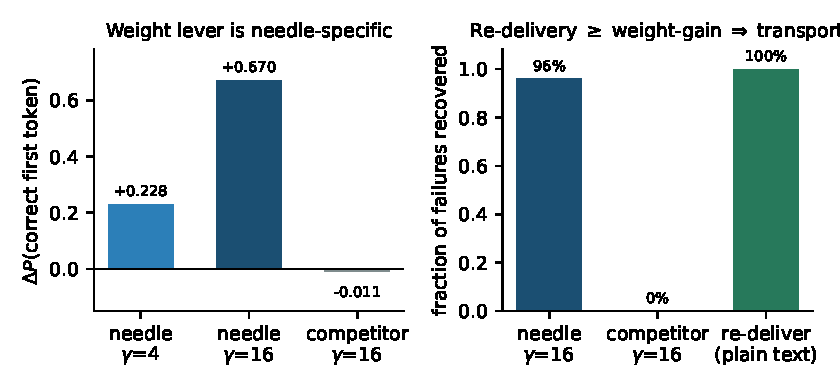
\includegraphics[width=0.86\textwidth]{figures/fig4_causal.pdf}
\caption{Causal probe (Llama-1B, 65K, $n{=}30$). \emph{Left:} multiplying the
needle's pre-softmax logits by $\gamma$ shifts $P(\text{correct})$ strongly
($+0.67$ at $\gamma{=}16$); boosting the winning-wrong competitor by the same factor
does not ($-0.011$) --- the lever is needle-specific and directional. \emph{Right:}
needle up-weighting recovers $96\%$ of the baseline-wrong cases (the report's
all-$P1$ denominator gives $80\%$), but plain re-delivery of the same fact recovers
$100\%\ge$ that --- so the weight manipulation buys nothing beyond delivery.}
\label{fig:causal}
\end{figure}

The needle-gain produces a large, needle-specific, directional argmax flip
(wrong$\to$correct; Fig.~\ref{fig:causal} left): attention weight \emph{does}
causally control which in-context information is used. But the pre-registered
discrimination is against an information-matched delivery control --- re-stating the
correct code in plain text near the question. That control recovers $100\%$, at least
as much as up-weighting ($\le$ the gain's $80$--$96\%$). By the pre-registered rule
(\textsc{transport} if the needle-gain effect is fully explained by re-delivery),
the correctness failure is \textbf{downstream of attention}: a delivery/salience
deficit plus the downstream weights, not a computation attention performs.
Mechanistically this \emph{closes} the class of memory schemes that would work by
redirecting attention flow, and leaves the weights path as the surviving lever. We
stress this verdict rests on the delivery explanation, not on a false ``inert'' ---
the weight effect is large and real ($+0.67$); it is simply redundant with delivery.

\section{Discussion}
\label{sec:discuss}

\paragraph{No compressor cliff.}
The practical consequence of \S\ref{sec:keff}--\ref{sec:cross} is that, above the
recency floor, the key budget is the wrong knob. Over $[1300,5200]$ a $4\times$ swing
is worth $\le 0.03$ accuracy at any tested $N$ and on three models. Top-$K$ retains
as well as dense up to the length where dense's own disambiguation fails. The ``safe
operating range'' is therefore set by coverage staying above the recency floor
($c\gtrsim 0.10$ keeps the answer selection-driven to $128\mathrm{K}$ in our 1B
sweep), not by hitting a budget threshold.

\paragraph{Retrieval is not reasoning, and the gap is in the weights.}
The cleanest object in the data is the selection/answer dissociation: selection
(retrieval) improves with budget and capacity; the answer is gated by
disambiguation, which lives in the weights and is what capacity buys. The causal
probe sharpens this --- even forcing the needle's weight up cannot manufacture an
answer beyond what mere delivery achieves. For practitioners targeting ``smarter''
on a fixed model, this says the lever is \emph{capacity or better delivery of
evidence}, not the sparsity budget; sparsity buys speed and length at iso-ability,
not ability.

\paragraph{Why a sparse method should report this.}
A sparse-attention paper has an incentive to attribute long-context failure to its
own budget (a knob it controls). The matched dense control shows the opposite:
within scope, the sparsifier is not the limiting factor. Reporting that honestly is
what makes the operating-range guidance trustworthy.

\section{Limitations}
\label{sec:limits}

\begin{itemize}
\item \textbf{Synthesis is out of scope.} Multi-hop chains floor on these bases
(1B and, in pilot, the 3B models in implicit two-hop), so this is a law for
\emph{retrieval selection under competition}, not for reasoning. Whether the budget
stays inert for synthesis on a model that does not floor is the immediate open gate.
\item \textbf{Boundary location vs.\ the null.} The headline (budget-inert,
no-$\Kcrit$, weights-bound) rests on within-run paired comparisons (immune to GPU
non-determinism), accRange an order of magnitude above seed noise, and cross-model
reproduction at $n{=}100$. Any claim about the \emph{exact} coverage onset $c^\ast$
at $128\mathrm{K}$ rests on single-seed $n{=}60$ runs and should be treated as
provisional pending a multi-seed repeat; we make no such claim in the headline.
\item \textbf{Scope.} Greedy, no chain-of-thought; semantic and near-duplicate
retrieval only; bf16 weights with fp32 softmax; $k_{\mathrm{window}}{=}64$ fixed
(all budgets $\gg$ this floor --- the window-dominated regime $N\!\cdot\!c$ near the
floor is not probed). $N$ is memory-bounded on the 3B models (Qwen $\le 65\mathrm{K}$,
Llama-3B $\le 49\mathrm{K}$ on 16\,GB), so the large-$N$ tail where 1B's
selected-yet-wrong fraction reaches $0.77$ is 1B-only here.
\item \textbf{Generality.} Three models and two families are a transfer result, not a
scaling law; cross-architecture confirmation is required before any ``law'' language.
\item \textbf{Intervention realism.} The causal probe lives in a reference attention
hook; production-kernel application of weight control is a separate engineering
question, and forcing attention is off-distribution (large-$\gamma$ degeneration is
expected and is itself informative).
\end{itemize}

\section{Conclusion}
\label{sec:conc}

Across Llama-3.2-1B, Qwen2.5-3B and Llama-3.2-3B, the absolute-key-budget
``Critical Semantic Capacity'' conjecture does not hold: the budget is inert over a
$4\times$ swing, no $\Kcrit$ emerges with capacity or across families, and top-$K$
sparse attention retains as well as dense. The long-context limit is the base model's
own length-driven disambiguation, which capacity improves; and a matched-control
causal probe shows attention here is (weighted) \emph{transport}, not computation ---
the correctness bottleneck is delivery plus the weights. Within the practical
operating regime there is no efficiency cliff in the compressor. The actionable lever
for ability is capacity or delivery; sparsity buys speed and length at iso-ability.

\section*{Reproducibility}
The repository accompanying this preprint contains every pre-registration, the raw
per-prompt logs for the three experiments, and \texttt{make\_figures.py}, which
recomputes all plotted numbers from the logs. Selection is exact
(Eq.~\ref{eq:thm1}); the cross-model kernel port is validated bitwise-exact against
a pure-PyTorch reference. Seed $20260531$; Llama-3.2-1B / Qwen2.5-3B / Llama-3.2-3B;
single RTX~4060~Ti.

\section*{Author contributions \& data}
E.V.\ designed the gates, ran the experiments, and performed the independent
numerical re-verification. D.V.\ contributed to design and analysis. Raw artifacts
and code are released under the repository's stated licenses.

\begin{thebibliography}{99}
\small
\bibitem{xiao2023streaming} G.\ Xiao et al. \emph{Efficient Streaming Language Models with Attention Sinks (StreamingLLM)}. ICLR, 2024.
\bibitem{zhang2023h2o} Z.\ Zhang et al. \emph{H2O: Heavy-Hitter Oracle for Efficient Generative Inference of LLMs}. NeurIPS, 2023.
\bibitem{li2024snapkv} Y.\ Li et al. \emph{SnapKV: LLM Knows What You are Looking for Before Generation}. NeurIPS, 2024.
\bibitem{xiao2024infllm} C.\ Xiao et al. \emph{InfLLM: Training-Free Long-Context Extrapolation with an Efficient Context Memory}. 2024.
\bibitem{tang2024quest} J.\ Tang et al. \emph{Quest: Query-Aware Sparsity for Efficient Long-Context LLM Inference}. ICML, 2024.
\bibitem{liu2024retrieval} D.\ Liu et al. \emph{RetrievalAttention: Accelerating Long-Context LLM Inference via Vector Retrieval}. NeurIPS, 2024.
\bibitem{singhania2024loki} P.\ Singhania et al. \emph{Loki: Low-Rank Keys for Efficient Sparse Attention}. NeurIPS, 2024.
\bibitem{deepseek2025v32} DeepSeek-AI. \emph{DeepSeek-V3.2: Sparse Attention (DSA)}. Technical report, 2025.
\bibitem{yuan2025nsa} J.\ Yuan et al. \emph{Native Sparse Attention (NSA)}. 2025.
\bibitem{tvtopk2025} \emph{A Mathematical Theory of Top-$k$ Sparse Attention via Total Variation Distance}. arXiv:2512.07647, 2025.
\bibitem{nativetopk2025} \emph{Native Top-$k$ Sparse Attention: Promises and Challenges}. arXiv:2512.03494, 2025.
\bibitem{criticalscaling2025} \emph{Critical Attention Scaling in Long-Context Transformers}. arXiv:2510.05554, 2025.
\bibitem{condensate2026} Ruiz Williams et al. \emph{The Condensate Theorem: Learned (not Architectural) Attention Concentration}. arXiv:2602.06317, 2026.
\bibitem{liu2024lost} N.\ F.\ Liu et al. \emph{Lost in the Middle: How Language Models Use Long Contexts}. TACL, 2024.
\bibitem{matchedcontrols2026} E.\ Vyaltsev, D.\ Vyaltsev. \emph{Matched-Magnitude Controls for Mechanistic Claims in Attention}. Zenodo, DOI 10.5281/zenodo.20261207, 2026.
\end{thebibliography}

\end{document}
